\documentclass[11pt,a4paper]{article}
\usepackage[margin=18mm]{geometry}
\usepackage{fontspec,unicode-math,amsmath,graphicx,booktabs,array,xcolor,fancyhdr}
\setmainfont{Latin Modern Roman}\setmathfont{Latin Modern Math}
\setlength{\parindent}{0pt}\setlength{\parskip}{8pt}
\pagestyle{fancy}\fancyhf{}\fancyfoot[L]{\small APD model comparison --- 6 October 2026}\fancyfoot[R]{\thepage}
\renewcommand{\headrulewidth}{0pt}
\begin{document}
{\LARGE\bfseries Two new tests: notebook background and Richard's four coefficients}\par
\textbf{Result.} The notebook's square background domain returns essentially the same optimum as the Stokes disk. Richard's exact four-coefficient approximation fits less well on held-out anisotropy and channel residuals. These tests use the same two intervals, calibrated channels, annulus, excitation law and ordered trajectory as the preceding comparisons.

\textbf{Test 1: relaxing only the background polarization constraint.}
\[
(B_0,B_{90},B_{45},B_{135})=\frac{B}{4}(1+f_a,1-f_a,1+f_b,1-f_b),
\qquad |f_a|,|f_b|\leq1.
\]
The extra Stokes restriction $f_a^2+f_b^2\leq1$ is removed. The total-background cap is kept at the same $0.95T_{\min}$ as the previous fixed-excitation additive fit, to isolate the domain change. This tests the original notebook's background family, not its old shape-only optimizer or preprocessing.

\textbf{Test 2: Richard's quoted approximation, without an additive term.}
\[
I_{m,j}=S_j+C_j\sqrt{S_j},\qquad C_j\in\mathbb R.
\]
Four coefficients are freely fitted, including either sign, with no imposed finite coefficient cap. Both tests retain one constant $a_0$ per interval and the prescribed circular-excitation dependence of $S_j$. The new parameters are 23 per interval for the square additive model and 24 for Richard's model.

{\small\begin{tabular}{llrrrr}\toprule
Window & Model & XY RMS & Channel RMS (\%) & BG/Tmax (\%) & $\theta$ (degrees)\\\midrule
30--31 s & Stokes additive & 0.0896 & 2.29 & 31.74 & 37.3--89.2 \\
30--31 s & Notebook-square additive & 0.0896 & 2.29 & 31.74 & 37.3--89.2 \\
30--31 s & Additive + sqrt extension & 0.0927 & 2.14 & 38.51 & 34.6--89.9 \\
30--31 s & Richard four-$C$ & 0.1041 & 2.56 & --- & 36.6--72.0 \\
10--11 s & Stokes additive & 0.0989 & 2.56 & 34.62 & 42.0--90.0 \\
10--11 s & Notebook-square additive & 0.0989 & 2.56 & 34.62 & 42.0--90.0 \\
10--11 s & Additive + sqrt extension & 0.1024 & 2.41 & 39.93 & 39.0--89.7 \\
10--11 s & Richard four-$C$ & 0.1057 & 2.71 & --- & 40.2--71.4 \\
\bottomrule\end{tabular}}

Scores are held-out. Channel residuals are normalized by measured total at each bin. Background is not inferred by Richard's four-$C$ approximation: the dash is not a claim of zero physical background. Angles are conditional on the fitted cone, not confidence intervals or known-angle accuracy.

\clearpage
{\Large\bfseries Fit overlays}\par
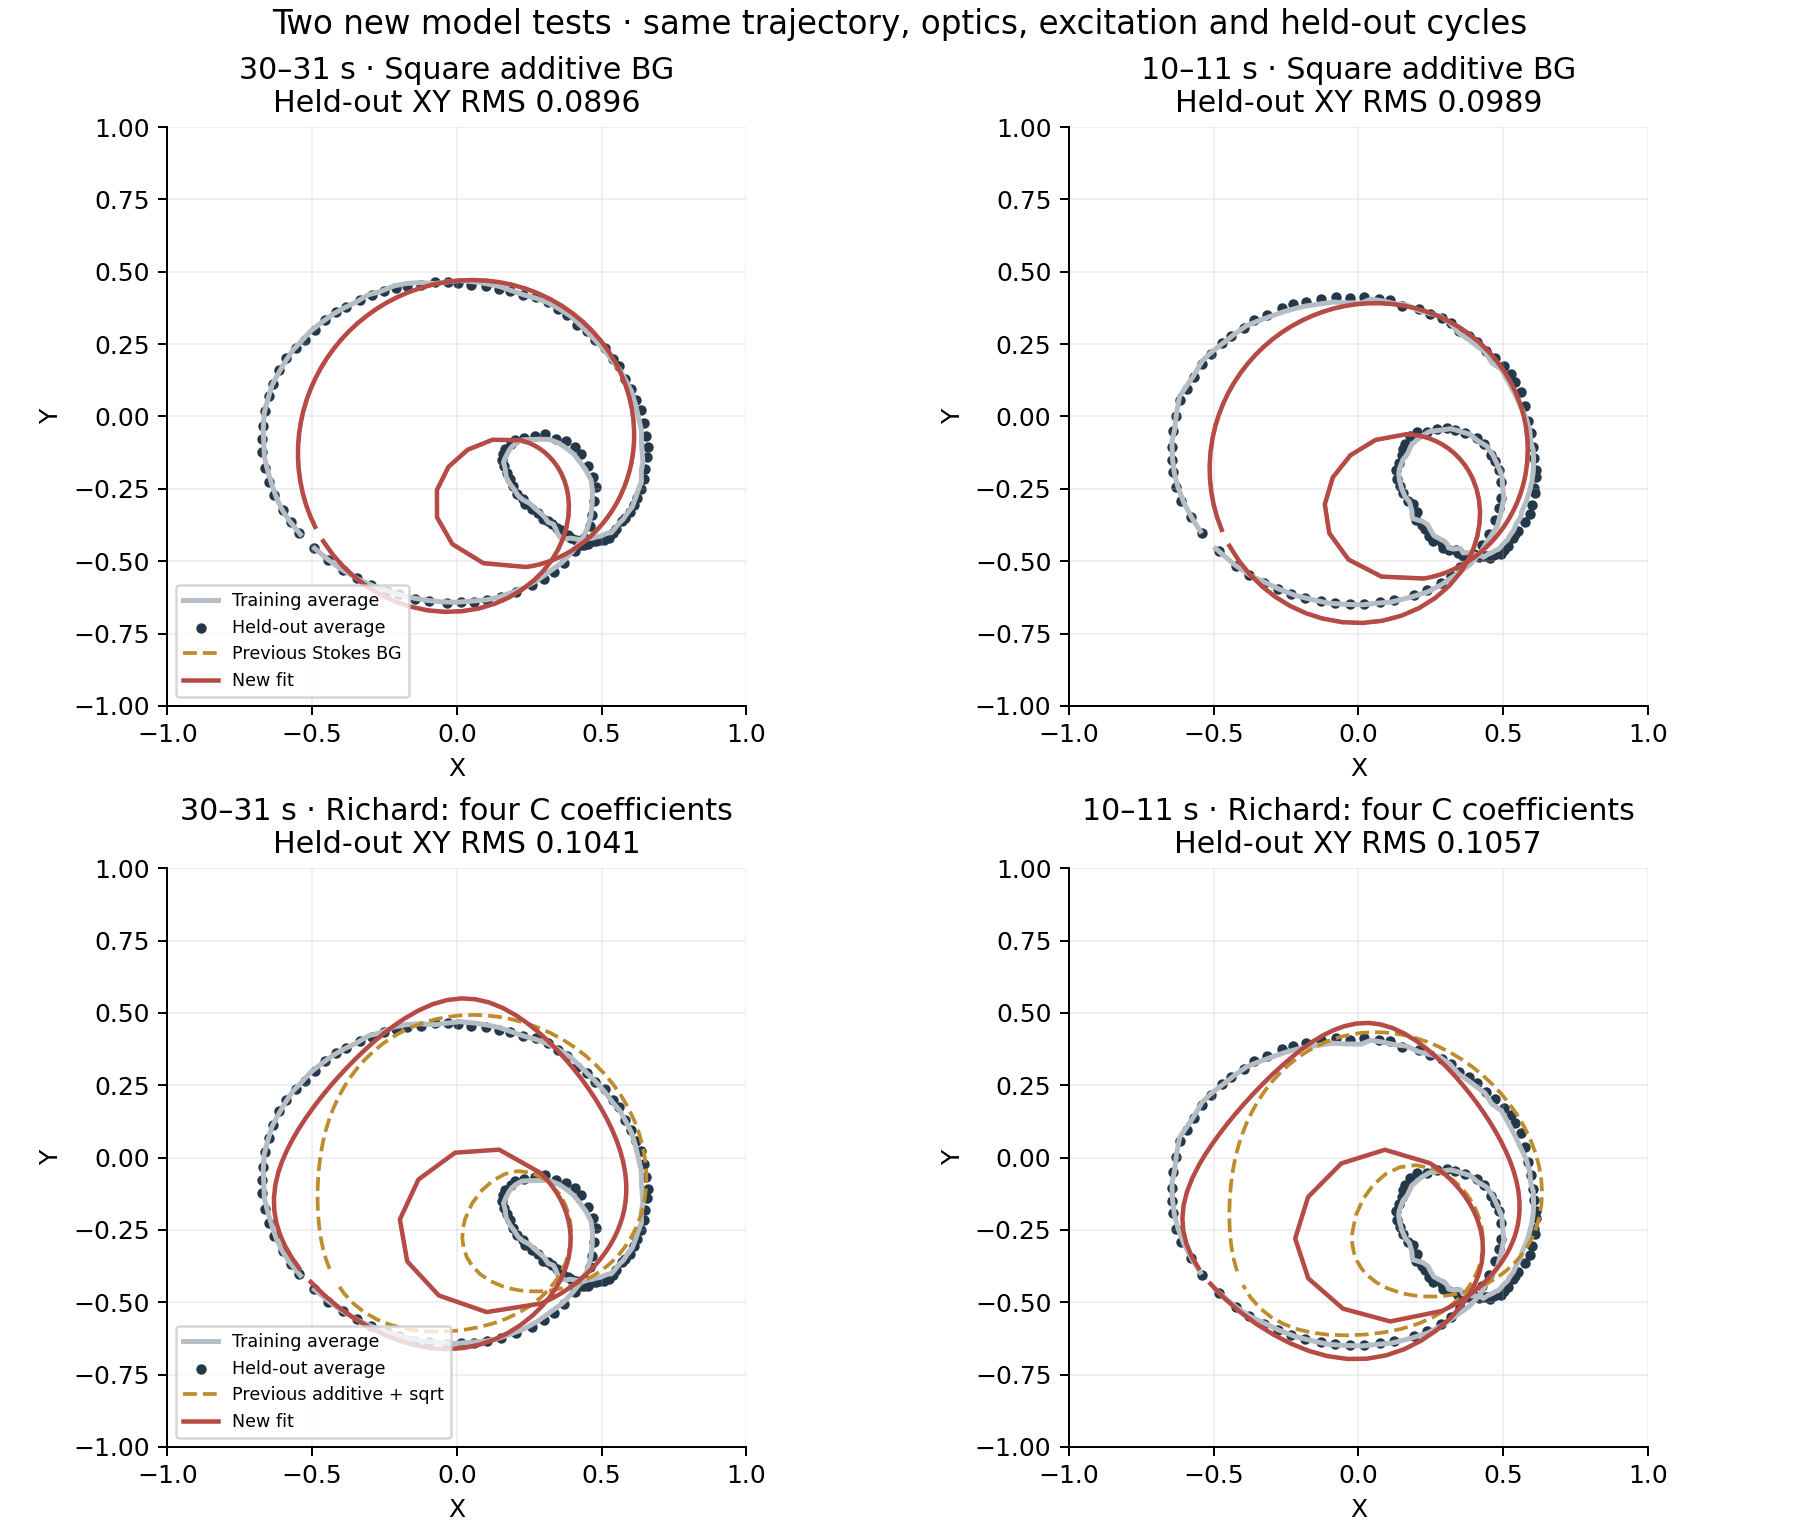
\includegraphics[width=\linewidth,height=.82\textheight,keepaspectratio]{two_new_fits.png}

The square-background prediction lies on top of the old Stokes prediction. The lower row distinguishes Richard's new four-$C$ fit from the previously fitted additive-plus-square-root extension. Every anisotropy axis spans $[-1,1]$.

\clearpage
{\Large\bfseries Power balance and angle consequences}\par
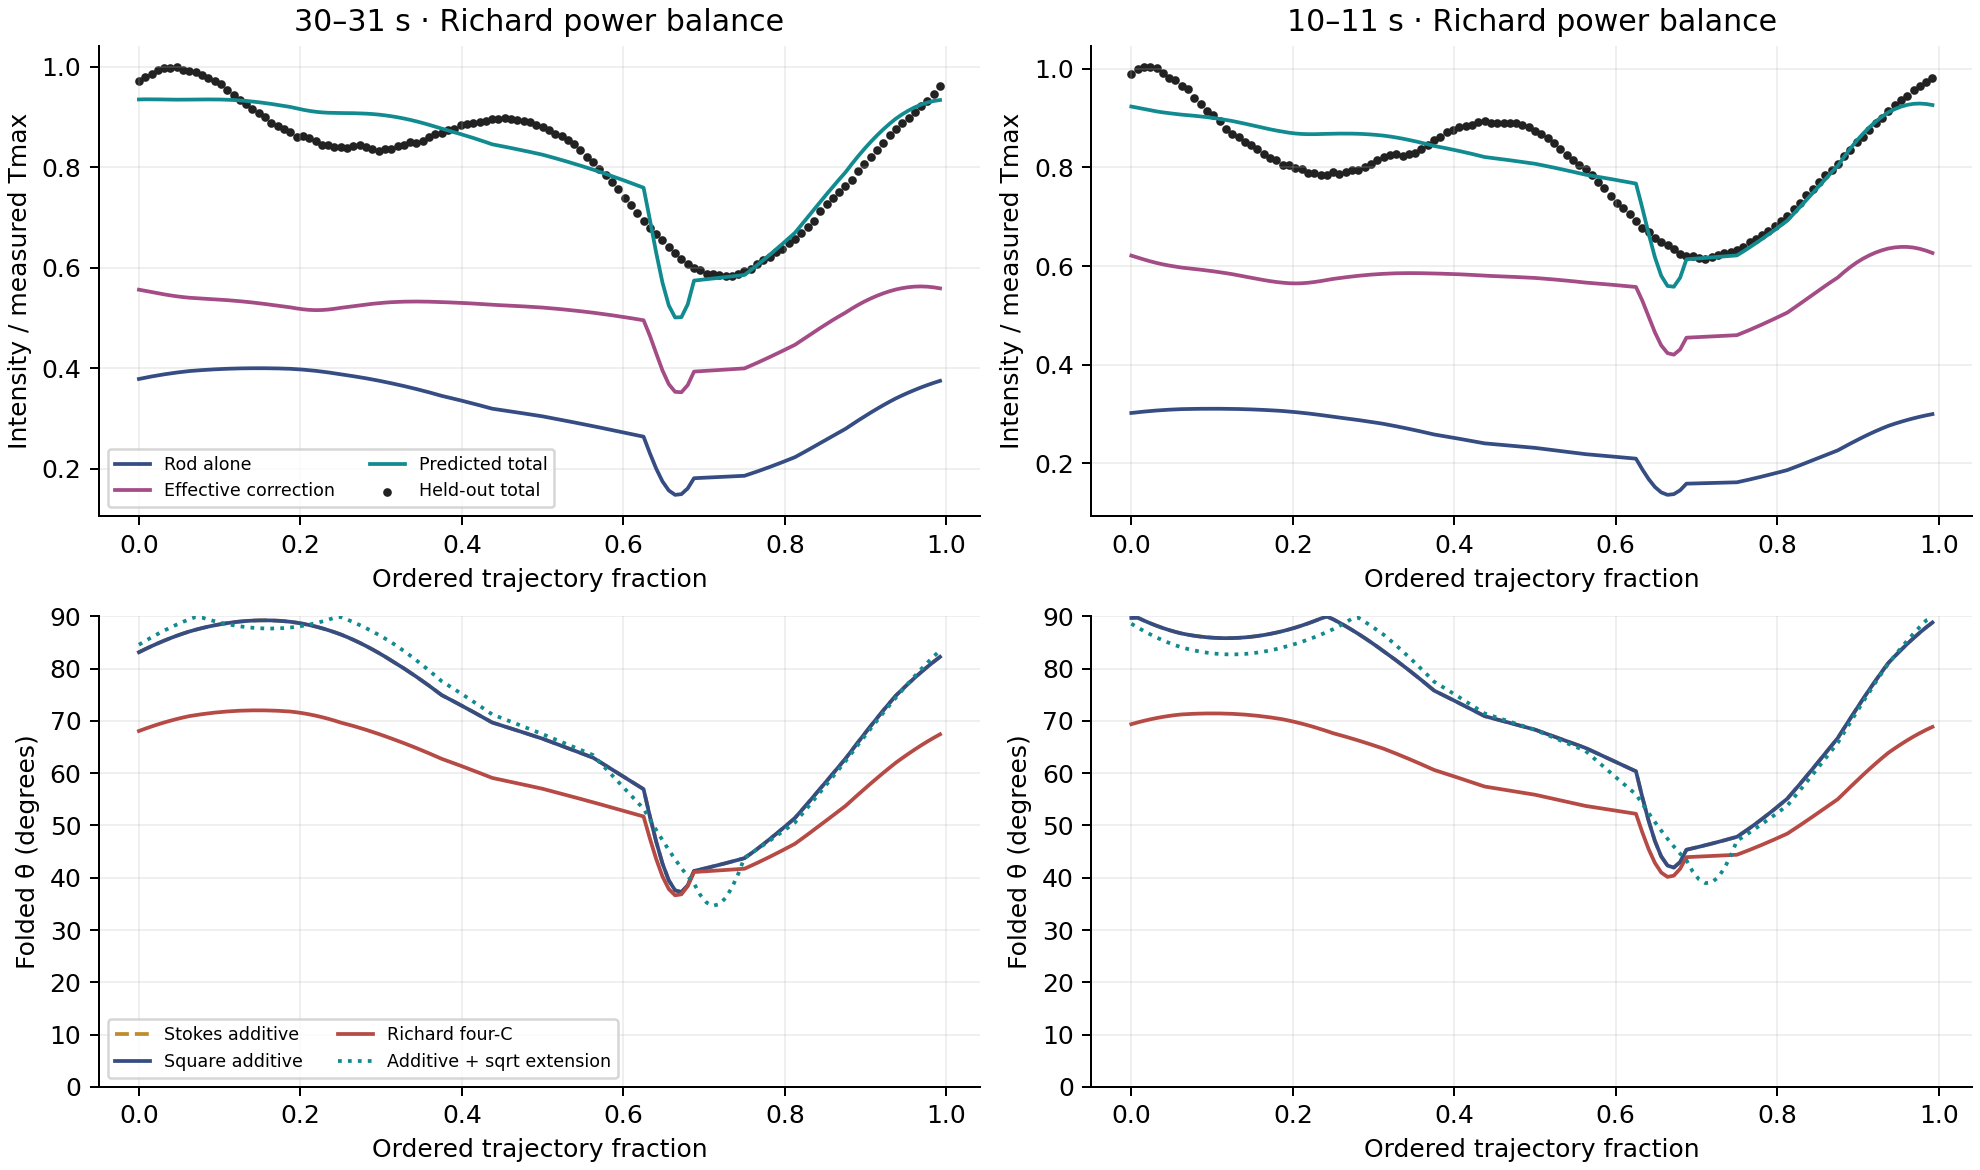
\includegraphics[width=\linewidth]{power_angles.png}

\textbf{Square versus disk.} The new optima have $(f_a,f_b)=(0.172,-0.405)$ and $(0.137,-0.452)$ for 30--31 s and 10--11 s. Their radii in the $(f_a,f_b)$ plane are $0.440$ and $0.472$, both well below one. The Stokes boundary was therefore not limiting these fixed-excitation additive fits. Background remains $31.74\%$ / $34.62\%$ of maximum total and the angle ranges are unchanged to numerical tolerance.

\textbf{Richard four-$C$.} All four selected coefficients are positive in both windows. The effective correction adds $35.2$--$56.3\%$ of maximum total at 30--31 s and $42.0$--$63.9\%$ at 10--11 s. These are signed correction terms evaluated along the fitted path, not constant background powers. The fitted $\theta$ ranges are $36.6$--$72.0^\circ$ and $40.2$--$71.4^\circ$.

Its held-out total-intensity RMS is slightly lower than additive-only (5.67\% versus 5.81\%, and 5.79\% versus 6.66\%), but its XY and channel RMS are worse. This is a tradeoff across observables, not improvement of the whole fit.

\clearpage
{\Large\bfseries Interpretation and checks}\par
\textbf{Can the fitted four-$C$ correction be interpreted literally as interference?}
For a given fitted rod signal, a physical coherent background obeys
\[
C_j=2\sqrt{B_{\mathrm{coh},j}}\,\rho_j,
\qquad |\rho_j|\leq1,
\qquad B_{\mathrm{coh},j}\geq C_j^2/4.
\]
If the selected coefficients are interpreted this way, the necessary summed coherent background is at least $23.4\%$ / $37.4\%$ of maximum measured total. Those are conditional bounds for this fitted decomposition, not estimates of the true background or proof that a common stationary field exists. They show that the omitted background-only power would not be negligible in that interpretation. These input traces had no independently measured optical-background subtraction.

Richard's equation remains a useful phenomenological approximation, particularly if background power has already been removed or is demonstrably negligible. The present results do not validate those assumptions for this recording. A coefficient acting as an effective correction may also absorb a different physical mismatch.

\textbf{Coefficient convention.} Normalize all four intensities by the common reference $T_{\mathrm{ref}}$, the larger of the two training maxima. Then $C'_j=C_j/\sqrt{T_{\mathrm{ref}}}$. In channel order $(0,90,45,135)$, the fitted coefficients are
\[
\mathbf C'_{30\mathrm{s}}=(0.5100,0.4381,0.3282,0.6096),
\]
\[
\mathbf C'_{10\mathrm{s}}=(0.6354,0.5467,0.3968,0.7986).
\]
The coefficients were fitted separately in the two intervals; a shared-coefficient hypothesis was not tested here.

\textbf{Numerical checks.} Ten starting points were used for each model/window (40 optimizations). All selected solutions terminated normally and predict positive channels at all 128 bins. Square-background starts return the same objective within numerical tolerance. The four-$C$ search has a worse local solution among the 30 s starts; the selected minimum is reported, not a certified global optimum. Brightness is not at its imposed numerical bounds. Direct quadratic inversion of each selected four-$C$ prediction recovers its modeled signal to numerical precision. No bins were dropped and no pointwise brightness freedom was introduced.

\textbf{What changes in the discussion.} The Stokes restriction does not explain the current additive-model mismatch. The exact four-$C$ proposal has now been tested and is not the better description under the present fixed-cone/excitation assumptions. This does not rule out effective interference models under other conditions or establish the true angles. This supplement supersedes the earlier note that Richard's exact model had not been run. No repository commit or push was made.
\end{document}
